\documentclass{subfile}

\begin{document}

\section{Primary Category}
	\begin{problem} Write down all the prime numbers in the range of $1$ to $50$.
	\end{problem}

	\begin{solution} $2, 3, 5, 7, 11, 13, 17, 19, 23, 29, 31, 37, 41, 43, 47$
	\end{solution}
	\begin{problem} Four people $A, B, C \text{ and } D$ have an average monthly income of $10000$ taka. First three of them have an
		average monthly income of $12000$ taka. Average income of first two of them is $15000$ taka. Find the
		monthly income of $B, C \text{ and } D$ if $A$ has a monthly income of 20000 taka.\\

	\end{problem}

	\begin{solution} Let $a, b, c, d$ denote their respective incomes. Then the given conditions are:
		\begin{align}
		&\frac{a+b+c+d}{4}=10000\Rightarrow a+b+c+d=40000\\
		&\frac{a+b+c}{3}=12000\Rightarrow a+b+c=36000\\
		&\frac{a+b}{2}=15000\Rightarrow a+b=30000\\
		& a=20000
		\end{align}
		(3) and (4) $\Rightarrow b=10000$\\
		(2) and (3) $\Rightarrow c=6000$\\
		(1) and (2) $\Rightarrow d=4000$\\

	\end{solution}

	\begin{problem} In the following figures a rectangular piece of paper $ABCD$ has been folded several times. First, the	side $CD$ was made to fall on the line $AD$. Point $E$ in figure (ii) represents the point $C$ after folding. In the next figure the portion $BF$ was made to fall on $EF$. Lastly, the side $AG$ was made to fall on $GH$. Find the lengths of $GJ, IJ, IE, ED, EH \text{ and } HF$. It is given that $AB = 8$ and $BC = 15$.
		\begin{figure}[h]
			\centering
			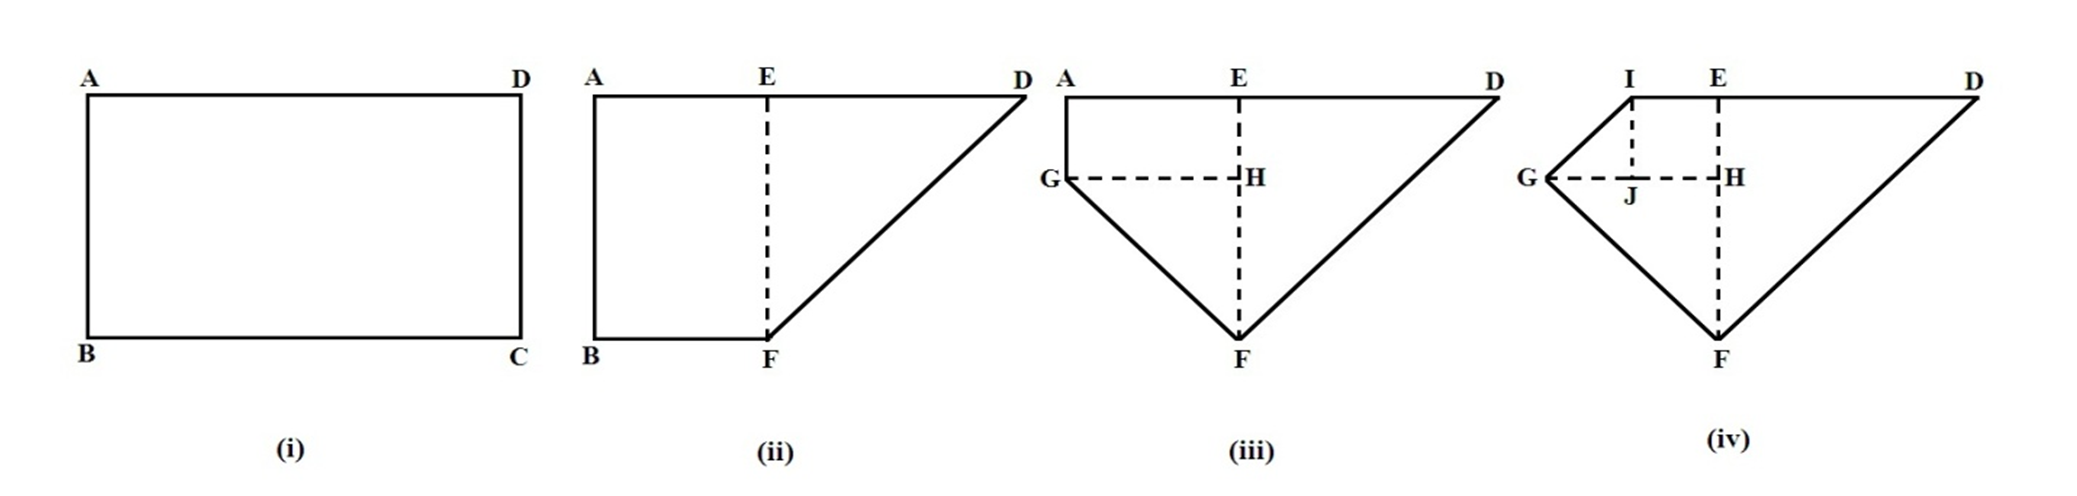
\includegraphics[width=1\linewidth]{Prob3.png}
		\end{figure}

	\end{problem}

	\begin{solution}
		\begin{align*}
		\textbf{Solution }&ED=EF=AB=8\\
		&HF=BF=AE=AD-ED=BC-ED=15-8=7\\
		&EH=EF-HF=AB-HF=8-7=1\\
		&GJ=GA=EH=1\\
		&IJ=EH=1\\
		&IE=AE-AI=BF-AI=HF-AI=HF-GJ=7-1=6
		\end{align*}

	\end{solution}

	\begin{problem} A circus party has the same number of lions as tigers. You asked to the owner of the circus the number
		of lions and tigers. He gave you the following information:
			\begin{enumerate}[i.]
				\item An elephant is enough to feed all the tigers and lions in the circus.
				\item Eighteen deers produce the same amount of meat as an elephant does.
				\item A lion eats twice as much as a tiger.
				\item One buffalo is enough to feed a lion and a tiger.
				\item A tiger will eat exactly the same amount of meat a deer has.
			\end{enumerate}
		Find the number of tigers and lions in that circus party.

	\end{problem}

	\begin{solution} Let the number of tigers(and lions)be $x$.
		\begin{enumerate}
			\item All of $2x$ animals eat in total $3x(\text{a single tiger's food})$.
			\item $3x(\text{a single tiger's food})=\text{an elephant}$.
			\item $ 3x(\text{a single tiger's food})=18 \text{ deer}$.
			\item $ 3x(\text{a single tiger's food})=18(\text{a single tiger's food})$
		\end{enumerate}
		So, $3x=18 \Rightarrow x=6$.
	\end{solution}


	\begin{problem} Surjo is four years old and he is learning to write numbers. His math notebook looks like a square grid with $20$ rows and $20$ columns. He usually writes the numbers from top to bottom and when one column is finished he starts writing along the next column. One day he starts writing the numbers from left to	right (along the rows). How many of the numbers will be placed in exactly the same place where it would have appeared if he had written along the columns?

	\end{problem}

	\begin{solution} Let $n$ be such a number which remained in the position in both of the writing methods.\\
		Let $x$ and $y$ be the row and column number of $n$, respectively, $1\leq x,y \leq 20$.\\
		Then following the order of the numbers in the vertical writing method,
		\begin{center}
			$n=20(y-1)+x$\\
		\end{center}


		\begin{flushleft}
			Again by the horizontal writing method,
			\begin{align*}
			&n=20(x-1)+y\\
			\therefore \text{ } &20(y-1)+x=n=20(x-1)+y\\
			\Rightarrow \text{ } &x=y
			\end{align*}
			So, $x$ must be equal to $y$ and there are $20$ such pairs. So they correspond to $20$ possible values for $n$.
		\end{flushleft}

	\end{solution}

	\begin{problem} In the following figure $BKLGNM, CMNHPO \text{ and } DOPIRQ$ are regular hexagons (all six sides of
		each hexagon are equal and so are the angles). $BKLGNM$ has an area of $24$ square units. What is the
		area of the rectangle $AFJE$?
		\begin{figure}[h]
			\centering
			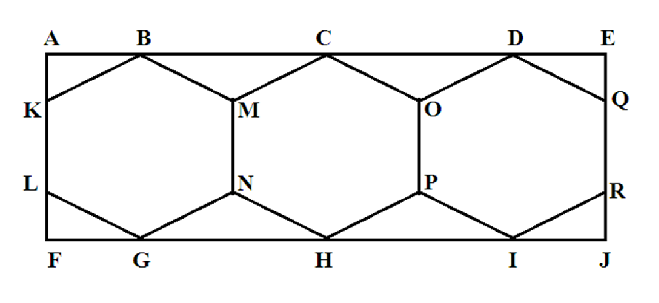
\includegraphics[width=0.7\linewidth]{Prob60.png}
		\end{figure}
	\end{problem}

	\begin{solution} Let the center of the hexagon $BKLGNM$ be $O \text{ and }\\ OB=OG=\frac{AF}{2}=a$. Then\\
		area$[BKLGNM]=6\times$ area$[OBK]$\\
		$\Rightarrow$ area$[OBK]=\frac{24}{6}=4$\\
		$\Rightarrow \frac{\sqrt{3}a^2}{4}=4$\\
		$\Rightarrow a=\frac{4}{\sqrt[4]{3}}$\\
		$\Rightarrow AF=\frac{8}{\sqrt[4]{3}}$\\
		Again, $\triangle OKL$ equilateral and with side-length $a$,
		so, altitude = $\frac{\sqrt{3}a}{2}=2\sqrt[4]{3}$\\
		So, $FJ=6\times \text{altitude of } \triangle OKL=12\sqrt[4]{3}$\\
		$\therefore \text{area} [AFJE]=AF\times FJ=96$

	\end{solution}

	\section{Junior Category}
	\begin{problem} A small country has a very simple language. People there have only two letters and all their words
	have exactly seven letters. Calculate the maximum number of words people can use in that country.

	\end{problem}

	\begin{solution} There are two possibilities for each letter. So $2^{7}$ possibilities for the $7$ letters. So they can use at most $2^{7}$ words.
    \end{solution}


	\begin{problem} In the following figures, the larger circles are identical and so are the smaller ones. In $(i)$ the circles
	have a common center and the lines $AD$ and $BC$ divide both the circles in four equal halves. The larger
	circle has an area of $100$ square meters. Find the area of the shaded region in figure$(ii)$.\\
	\begin{figure}[h]
		\centering
		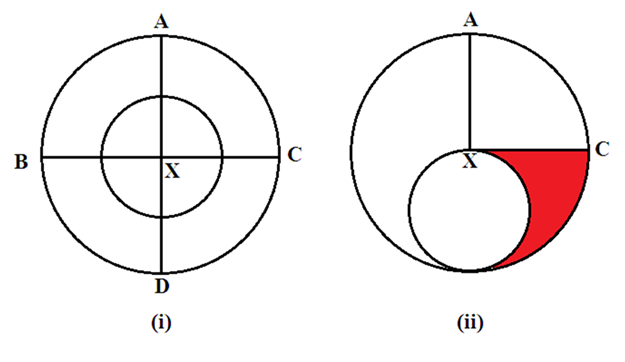
\includegraphics[width=0.7\linewidth]{Prob2.png}
	\end{figure}

	\end{problem}


	\begin{solution}
	$\text{area}[\text{circle} ABCD]=100 \Rightarrow \text{area}[XDC]=25$\\
	$\text{radius of ABCD}=\sqrt{\dfrac{\text{area}[ABCD]}{\pi}}=\sqrt{100/\pi}=2\times$radius of small circle\\
	So, $\text{area}[\text{small circle}]=\pi \left(\dfrac{5}{\pi}\right)^{2}=\frac{25}{\pi}$
	\begingroup
	\setlength{\abovedisplayskip}{0pt}
	\begin{flalign*}
		\therefore \text{area of the shaded region} &=\text{area}[XDC]-\dfrac{\text{area}[\text{small circle}]}{2} &\\
		&= 25 - \dfrac{\dfrac{25}{\pi}}{2}\\
	\end{flalign*}
	\endgroup
	\end{solution}

	\begin{problem} A circus party has the same number of lions as tigers. You asked to the owner of the circus the number
		of lions and tigers. He gave you the following information:
		\begin{enumerate}[i.]
			\item An elephant is enough to feed all the tigers and lions in the circus.
			\item Eighteen deers produce the same amount of meat as an elephant does.
			\item A lion eats twice as much as a tiger.
			\item One buffalo is enough to feed a lion and a tiger.
			\item A tiger will eat exactly the same amount of meat a deer has.
		\end{enumerate}
		Find the number of tigers and lions in that circus party.

	\end{problem}

	\begin{solution} Let the number of tigers(and lions)be $x$.
		\begin{enumerate}
			\item All of $2x$ animals eat in total $3x(\text{a single tiger's food})$.
			\item $3x(\text{a single tiger's food})=\text{an elephant}$.
			\item $ 3x(\text{a single tiger's food})=18 \text{ deer}$.
			\item $ 3x(\text{a single tiger's food})=18(\text{a single tiger's food})$
		\end{enumerate}
		So, $3x=18 \Rightarrow x=6$.
	\end{solution}


	\begin{problem} In the following figure $BKLGNM, CMNHPO \text{ and } DOPIRQ$ are regular hexagons (all six sides of
	each hexagon are equal and so are the angles). $BKLGNM$ has an area of $24$ square units. What is the
	area of the rectangle $AFJE$?
	\begin{figure}[h]
		\centering
		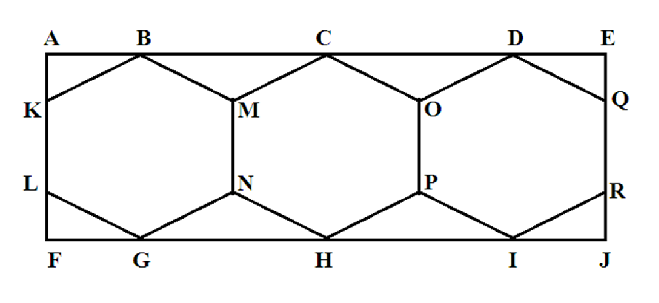
\includegraphics[width=0.7\linewidth]{Prob4.png}
	\end{figure}

	\end{problem}
    \begin{solution} Let the center of the hexagon $BKLGNM$ be $O \text{ and }\\ OB=OG=\dfrac{AF}{2}=a$. Then\\
	area$[BKLGNM]=6\times$ area$[OBK]$\\
	$\Rightarrow$ area$[OBK]=\dfrac{24}{6}=4$\\
	$\Rightarrow \dfrac{\sqrt{3}a^2}{4}=4$\\
	$\Rightarrow a=\dfrac{4}{\sqrt[4]{3}}$\\
	$\Rightarrow AF=\dfrac{8}{\sqrt[4]{3}}$\\
	Again, $\triangle OKL$ equilateral and with side-length $a$,
	so, altitude = $\dfrac{\sqrt{3}a}{2}=2\sqrt[4]{3}$\\
	So, $FJ=6\times \text{altitude of } \triangle OKL=12\sqrt[4]{3}$\\
	$\therefore \text{area} [AFJE]=AF\times FJ=96$
	\end{solution}


	\begin{problem} In a party, boys shake hands with girls only but each girl shakes hands with everyone else. If there are
		total $40$ handshakes, find the number (more than one) of boys and girls in the party.


	\end{problem}



	\begin{solution}
		Let the number of boys in the party be $x$ and the number of girls be $y$. Then each boy shakes hands exactly $y$ times and each girl shakes hands $y+(x-1)$ times. So the total number of handshakes will be $xy+y(y+x-1)=y(2x+y-1)$
		$\therefore y(2x+y-1)=40$\\
		Now a little checking for  $y$ over the factors of $40$ shows us that only for $y=5(y>1)$ we get a positive integral value for $x(=8)$.\\
	\end{solution}

	\begin{problem} $ABCD$ is a parallelogram, where $\angle ACB=80^{\circ} ,$ $\angle ACD=20^{\circ}$. $P$ is a point on $AC$ such that, $\angle ABP=20^{\circ}$ and $Q$ is a point on $AB$ such that $\angle ACQ=30^{\circ}$. Find the magnitude of the angle determined by the lines $CD$ and $PQ$.
	\end{problem}

	\begin{solution}Let $PQ$ meet $CD$ at $K$ and the parallel from $P$ to $BC$ meet $AB$ at $F$. Let $CF$ meet $BP$ at $G$.
	Since $\triangle BCG$ is equilateral, $BG=BC$. Since $\triangle CBQ$ is isosceles $BQ=BC$. Hence $\triangle BGQ$ is isosceles,
	\begin{center}
		$\angle BGQ=80^{\circ},$ $\angle FGQ=40^{\circ}$
	\end{center}
	Since $\angle QFG=40^{\circ}$, $\triangle FQG$ is isosceles and $FQ=QG$. Also $PF=PG$. Hence $\triangle GPQ\cong \triangle FPQ, PQ$ bisects $\angle FPG$, and $\angle QPB=30^{\circ}$.
	Now $\angle CKQ=\angle CPQ-\angle KCP=(\angle CPB+\angle BPQ)-\angle KCP=(40^{\circ}+30^{\circ})-20^{\circ}=50^{\circ}$.\\
	\begin{figure}[h]
		\centering
		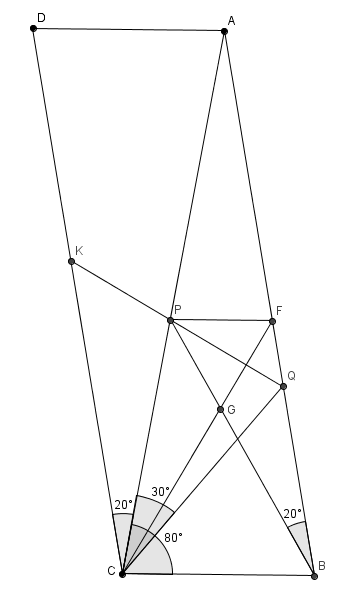
\includegraphics[width=0.4\linewidth, height=0.35\textheight]{Prob6.PNG}
	\end{figure}

	\end{solution}
	\section{Secondary Category}
	\begin{problem}
		A crime is committed during the hortal. There are four witnesses. The witnesses are logicians and make the following statements.
		\begin{itemize}
			\item Witness one says exactly one of the witnesses are liar
			\item Witness one says exactly two
			of the witnesses are liar
			\item Witness one says exactly three of the witnesses are liar
			\item Witness one says exactly four of the witnesses are liar
		\end{itemize}
		Assume that each of the statements are true or false. Find the number of liar witnesses.
	\end{problem}
		\begin{solution} All the $4$ witnesses provided $4$ different kind of informations and any two of them cannot be true at the same time. So there can be at most $1$ truthful. Again all $4$ of them cannot be liar otherwise the $4$th person will be truthful. So there are exactly $3$ liars.

		\end{solution}


		\begin{problem}\label{prb:1.3.2}
			There were $36$ participants in a BdMO event. Some of the participants shook hand with each other. No two of them shook hands with each more than once. It was found that no two participants with the same number of handshakes made, had shaken hands each other. Find the maximum number of handshakes at the party.
		\end{problem}

		\begin{solution}

			Suppose that the number of participants who shook hands with exactly $i$ other participants is $f(i)$. Then, due to the given condition, $f(i)\leq 36-i$. Now, the total number of handshakes is $\dfrac{1}{2}\sum\limits_{i=0}^{35}if(i)$. Thus,

			\begin{align*}
				\dfrac{1}{2}\sum\limits_{i=0}^{35} i\cdot f(i) & \leq \dfrac{1}{2}\sum\limits_{i=0}^{35}i(36-i)=3885
			\end{align*}

			Thus the maximum number of handshakes at the party is $3885$. It's left to the reader to find an appropriate construction with $3885$ handshakes.

		\end{solution}

		\begin{problem}
			A tetrahedron is a polyhedron composed of $4$ triangular faces. Faces $ABC$ and $BCD$ of tetrahedron $ABCD$ meet at and angle of $\frac{\pi}{6}$. The area of $\triangle ABC$ and $\triangle BCD$ are $120$ and $80$ resp. where $BC=10$. What is the volume of the tetrahedron? (The volume of a tetrahedron is one third the area of it's base times its height)
		\end{problem}
		\begin{solution} Let $P$ and $Q$ be the projection of $A$ on the plane $BCD$ and line $BC$ resp.\\

			Then $$(ABC)=\dfrac{1}{2}\times BC\times AQ \Longrightarrow AQ=\dfrac{2\times 120}{10}=24$$

			Again $\angle AQP=30^{\circ}$ and $\angle APQ=90^{\circ}$. So $AP=AQ\times \sin 30^{\circ}=\dfrac{24}{2}=12$

			$\therefore$ volume of tetrahedron $ABCD=\dfrac{1}{3}\times (BCD)\times AP=\dfrac{1}{3}\times 80 \times 12=320$.

		\end{solution}

		\begin{problem}
			Trapezoid $ABCD$ has sides $AB=92,BC=50,CD=19,AD=70$.The side $AB$ is parallel to $CD$. A circle with center $P$ on $AB$ is drawn tangent to $BC$ and $AD$. Given that $AP=\frac{m}{n}$ where $m$ and $n$ are coprime positive integers. Find $m+n$?
		\end{problem}

		\begin{solution} Let the circle touches $AC$ and $BD$ at $Q$ and $R$ resp and $AD\cap BC=S$.\\
			Then $PQ\perp BC$ and $PR\perp AD$.
			So
		\begin{eqnarray*}
			PQ=PR
			& \Longrightarrow & PB.\sin \angle PBQ=PA.\sin \angle PAR\\
			& \Longrightarrow & \frac{PB}{PA}=\frac{\sin \angle BAS}{\sin \angle ABS}\\
			& \Longrightarrow & \dfrac{AB-PA}{PA}=\dfrac{BS}{AS}\\
			& \Longrightarrow & \dfrac{92}{PA}-1=\dfrac{BC}{AD}\\
			& \Longrightarrow & \dfrac{92}{PA}=1+\dfrac{50}{70}=\dfrac{12}{7}\\
			& \Longrightarrow & PA=\dfrac{92\times 7}{12}=\dfrac{161}{3}
		\end{eqnarray*}

			$\therefore m+n=164$.

		\end{solution}

		\begin{problem}
			In $\triangle ABC$, $A',B',C'$ are on sides $BC,CA,AB$ resp. Also $AA',BB',CC"$ are concurrent at $O$. Also, $\dfrac{AO}{OA'}+\dfrac{BO}{OB'}+\dfrac{CO}{OC'}=92$. Find $\dfrac{AO}{OA'}\dfrac{BO}{OB'}\dfrac{CO}{OC'}$.
		\end{problem}

		\begin{solution} Let $(BOC)=p,(COA)=q$ and $(AOC)=r$.
			$$\dfrac{AO}{OA'}=\dfrac{(ABO)}{(OBA')}=\dfrac{(ACO)}{(OCA')}=\dfrac{(ABO)+(ACO)}{(OBA')+(OCA')}=\dfrac{q+r}{p}$$
			Similarly $\dfrac{BO}{OB'}=\frac{r+p}{q}$  and  $\dfrac{CO}{OC'}=\dfrac{p+q}{r}$.\\
			Therefore $\dfrac{AO}{OA'}+\dfrac{BO}{OB'}+\dfrac{CO}{OC'}=92$ implies\\ $$\dfrac{q+r}{p}+\dfrac{r+p}{q}+\dfrac{p+q}{r}=\frac{\sum_{cyc}^{}{q^2r+qr^2}}{pqr}=92$$



			So \begin{eqnarray*}
				\dfrac{AO}{OA'}\dfrac{BO}{OB'}\dfrac{CO}{OC'}
				& = & \dfrac{q+r}{p}\times \dfrac{r+p}{q}\times \dfrac{p+q}{r}\\
				& = & \dfrac{(\sum_{cyc}^{}{q^2r+qr^2})+2pqr}{pqr}\\
				& = & 92+2\\
				& = & 94
			\end{eqnarray*}

		\end{solution}

	\section{Higher Secondary Category}
	\begin{problem}
		A crime is committed during the hortal. There are four witnesses. The witnesses are logicians and make the following statements.
		\begin{itemize}
			\item Witness one says exactly one of the witnesses are liar
			\item Witness one says exactly two
			of the witnesses are liar
			\item Witness one says exactly three of the witnesses are liar
			\item Witness one says exactly four of the witnesses are liar
		\end{itemize}
		Assume that each of the statements are true or false. Find the number of liar witnesses.
	\end{problem}

		\begin{solution} All the $4$ witnesses provided $4$ different kind of informations and any two of them cannot be true at the same time. So there can be at most $1$ truthful. Again all $4$ of them cannot be liar otherwise the $4$th person will be truthful. So there are exactly $3$ liars.

		\end{solution}

		\begin{problem}
			Let $N$ be the number of pairs $(m,n)$ of integers that satisfy the equation $m^2+n^2=m^3$. Is $N$ finite or infinite. If $N$ is finite, find the cardinality of $N$.
		\end{problem}
		\begin{solution}
			$m^2+n^2=m^3 \Longrightarrow n^2=m^2(m-1)$. Now if we take $m=k^2+1$ where $k\in \mathbb{N}$, then $(m,n)=(k^2+1,k(k^2+1))$ is a valid solution. As there are infinite choices of $k$, it has infinite solutions. Hence $N$ is infinite.
		\end{solution}

		\begin{problem}
			Let $n$ be a positive integer. Consider the polynomial $p(x)=x^2+x+1$. What is the remainder of $x^3$ when divided by $x^3$. For what $n\in \mathbb{N}$ is $x^{2n}+x^n+1$ divisible by $p(x)$?
		\end{problem}
		\begin{solution}
			\begin{align*}
				x^3-1 & =(x-1)(x^2+x+1)\\
					  & \equiv 0 \pmod{p(x)}\\
				x^3	  & \equiv 1\pmod{p(x)}
			\end{align*}
			Notice that,
				\begin{align*}
					x^{2n}+x^n+1
					&	\equiv
						\begin{cases}
							\left(x^3\right)^{\frac{2n}{3}}+\left(x^3\right)^{\frac{n}{3}}+1 \equiv 1+1+1 \equiv 3\pmod{p(x)}
							\text{ if }3|n\\
							x^2+x+1\equiv0\pmod{p(x)}\text{ if }3\nmid n
						\end{cases}
				\end{align*}
			The second case is true because $\{2n,n\}\equiv\{1,2\}\pmod 3$.
		\end{solution}

		\begin{problem}
			There were $36$ participants in a BdMO event. Some of the participants shook hand with each other. No two of them shook hands with each more than once. It was found that no two participants with the same number of handshakes made, had shaken hands each other. Find the maximum number of handshakes at the party.
		\end{problem}

		\begin{solution}
			Same as \eqref{prb:1.3.2}.
		\end{solution}

		\begin{problem}
			A tetrahedron is a polyhedron composed of $4$ triangular faces. Faces $ABC$ and $BCD$ of tetrahedron $ABCD$ meet at and angle of $\frac{\pi}{6}$. The area of $\triangle ABC$ and $\triangle BCD$ are $120$ and $80$ resp. where $BC=10$. What is the volume of the tetrahedron? (The volume of a tetrahedron is one third the area of it's base times its height)
		\end{problem}
		\begin{solution} Let $P$ and $Q$ be the projection of $A$ on the plane $BCD$ and line $BC$ respectively. Then
				\begin{align*}
					(ABC)=\dfrac{1}{2}\times BC\times AQ \Longrightarrow AQ=\dfrac{2\times 120}{10}=24
				\end{align*}

			Again $\angle AQP=30^{\circ}$ and $\angle APQ=90^{\circ}$. So $AP=AQ\times \sin 30^{\circ}=\dfrac{24}{2}=12$

			$\therefore$ volume of tetrahedron $ABCD=\dfrac{1}{3}\times (BCD)\times AP=\dfrac{1}{3}\times 80 \times 12=320$.

		\end{solution}

		\begin{problem}
			Trapezoid $ABCD$ has sides $AB=92,BC=50,CD=19,AD=70$.The side $AB$ is parallel to $CD$. A circle with center $P$ on $AB$ is drawn tangent to $BC$ and $AD$. Given that $AP=\frac{m}{n}$ where $m$ and $n$ are coprime positive integers. Find $m+n$?
		\end{problem}

		\begin{solution} Let the circle touches $AC$ and $BD$ at $Q$ and $R$ resp and $AD\cap BC=S$.\\
			Then $PQ\perp BC$ and $PR\perp AD$.
			So
		\begin{eqnarray*}
			PQ=PR
			& \Longrightarrow & PB.\sin \angle PBQ=PA.\sin \angle PAR\\
			& \Longrightarrow & \frac{PB}{PA}=\frac{\sin \angle BAS}{\sin \angle ABS}\\
			& \Longrightarrow & \dfrac{AB-PA}{PA}=\dfrac{BS}{AS}\\
			& \Longrightarrow & \dfrac{92}{PA}-1=\dfrac{BC}{AD}\\
			& \Longrightarrow & \dfrac{92}{PA}=1+\dfrac{50}{70}=\dfrac{12}{7}\\
			& \Longrightarrow & PA=\dfrac{92\times 7}{12}=\dfrac{161}{3}
		\end{eqnarray*}

			$\therefore m+n=164$.

		\end{solution}

		\begin{problem}
			In $\triangle ABC$, $A',B',C'$ are on sides $BC,CA,AB$ resp. Also $AA',BB',CC"$ are concurrent at $O$. Also, $\dfrac{AO}{OA'}+\dfrac{BO}{OB'}+\dfrac{CO}{OC'}=92$. Find $\dfrac{AO}{OA'}\dfrac{BO}{OB'}\dfrac{CO}{OC'}$.
		\end{problem}

		\begin{solution} Let $(BOC)=p,(COA)=q$ and $(AOC)=r$.
			$$\dfrac{AO}{OA'}=\dfrac{(ABO)}{(OBA')}=\dfrac{(ACO)}{(OCA')}=\dfrac{(ABO)+(ACO)}{(OBA')+(OCA')}=\dfrac{q+r}{p}$$\\
			Similarly $\dfrac{BO}{OB'}=\frac{r+p}{q}$  and  $\dfrac{CO}{OC'}=\dfrac{p+q}{r}$.\\
			Therefore $\dfrac{AO}{OA'}+\dfrac{BO}{OB'}+\dfrac{CO}{OC'}=92$ implies\\ $$\dfrac{q+r}{p}+\dfrac{r+p}{q}+\dfrac{p+q}{r}=\frac{\sum_{cyc}^{}{q^2r+qr^2}}{pqr}=92$$


		So \begin{eqnarray*}
			\dfrac{AO}{OA'}\dfrac{BO}{OB'}\dfrac{CO}{OC'}
			& = & \dfrac{q+r}{p}\times \dfrac{r+p}{q}\times \dfrac{p+q}{r}\\
			& = & \dfrac{(\sum_{cyc}^{}{q^2r+qr^2})+2pqr}{pqr}\\
			& = & 92+2\\
			& = & 94
		\end{eqnarray*}

		\end{solution}

		\end{document}